\section{Introduction 10\%}
Describe the problem you are working on, why it's important, and an overview of your results.\\
Image processing and its related algorithms are used to process digital images. Although it may seem recent technology, many of the techniques were developed in the 1960s. However, computers were expensive at this time and the digital imaging process required too much resources for many to even consider. The situation changed in the 1970s, when digital image processing began to be used massively as cheaper computers and dedicated hardware became available. With the accessibility to faster computers in the 2000s, digital image processing has become the most common form of image processing, able to compute different tasks such as image classification, video and real time detection. With the birth and growth of intelligent systems, Computer vision is increasingly used in the field of intelligent transport, which includes the subject of this paper: traffic sign recognition. It can be seen as a third eye which concerns a wide area of usages such as self-driving cars. These systems are typically based on detecting a region of interest (ROI), in which the traffic sign is located, recognising typical characteristics such as colour and geometric form. These information provide crucial visual details in order to understand the proper driving conditions. For example, they inform about speed limits, drivable lanes, obstacles, temporary situations, roadway access, restrictive areas, etc. Reasons why they are designed to be easily detectable, recognizable and interpretable by humans.
\begin{figure}[h]
	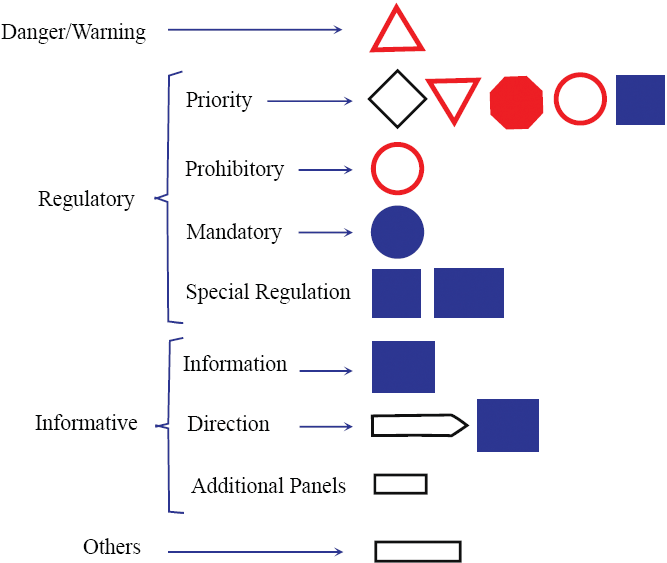
\includegraphics[width=\linewidth]{Res/Immagini/european-traffic-signs.PNG}	
	\caption{European Traffic Sign Categories}
\end{figure}


The application developed includes not only the standard functionality of image processing but also image and video detection and image classification. The original idea of combining different processes shows how powerful this tool can be. This is made possible through a long and accurate training process, based on a dataset of normalized traffic signs.\\ The process starts with the detection stage for the input image or video. This phase exploits the YOLO library for object detection which detects the area where a possible traffic sign is located and draws the so-called bounding boxes around it. We chose YOLO because of its main feature of being significantly faster than other framework, trading a bit of accuracy. Once the first step is completed, each object is passed to the classifier which is in charge to find out the correct label for the image. For this purpose we lean on Keras, a deep-learning framework.
%------------------------------------------------------------------------